
\subsubsection{6.1 Key Findings}

\textbf{Extension of HT-SR to Attention Mechanisms.} Heavy-tailed exponents were computed for 53 ViT models using the Hill estimator on attention weight matrices. All processed models exhibited heavy-tailed distributions with $\alpha$ values in the [2.20, 18.92] range, broader than the [2, 6] range typically reported for CNNs.

\textbf{Training Origin Appears to Dominate Variance.} The 12-fold variance reduction through family stratification suggests that training provenance may be the primary variance driver rather than architectural differences. Models sharing training origin (google/vit-*) show consistent $\alpha$ values ($\sigma$ = 0.24) regardless of size variants (base, large, different patch sizes).

\textbf{Task-Specific Fine-Tuning Creates Outliers.} Models fine-tuned for specialized tasks exhibit extreme $\alpha$ values (>10), reflecting genuine distributional shifts from the base model weights.

\subsubsection{6.2 Limitations}

\textbf{Sample Size Below Target.} 53 of 100 target models were processed (53\% success rate). The primary cause was incompatibility between timm-format models and HuggingFace Transformers loading, not issues with $\alpha$ computation itself.

\textbf{Single Family Tested for Within-Family Variance.} Only the google/vit-* family (n=6) had sufficient samples for reliable within-family variance estimation. Other families had insufficient samples.

\textbf{Downstream Hypotheses Not Tested.} The gate failure ($\sigma$ > 0.5) blocked testing of downstream hypotheses regarding cross-architecture prediction transfer.

\textbf{Model Loading Failure Rate.} The 47\% failure rate introduces possible survivorship bias, though failures were due to technical format issues rather than $\alpha -related$ selection.

\subsubsection{6.3 Implications}

For practitioners seeking weight-based model selection across diverse hubs, these results suggest that:

\begin{enumerate}
\item Heavy-tailed analysis is technically feasible for ViT architectures
\item Direct cross-model comparison without controlling for training origin may be unreliable
\item Within-family comparisons may achieve bounded variance suitable for ranking
\end{enumerate}

\begin{figure}[htbp]
\centering
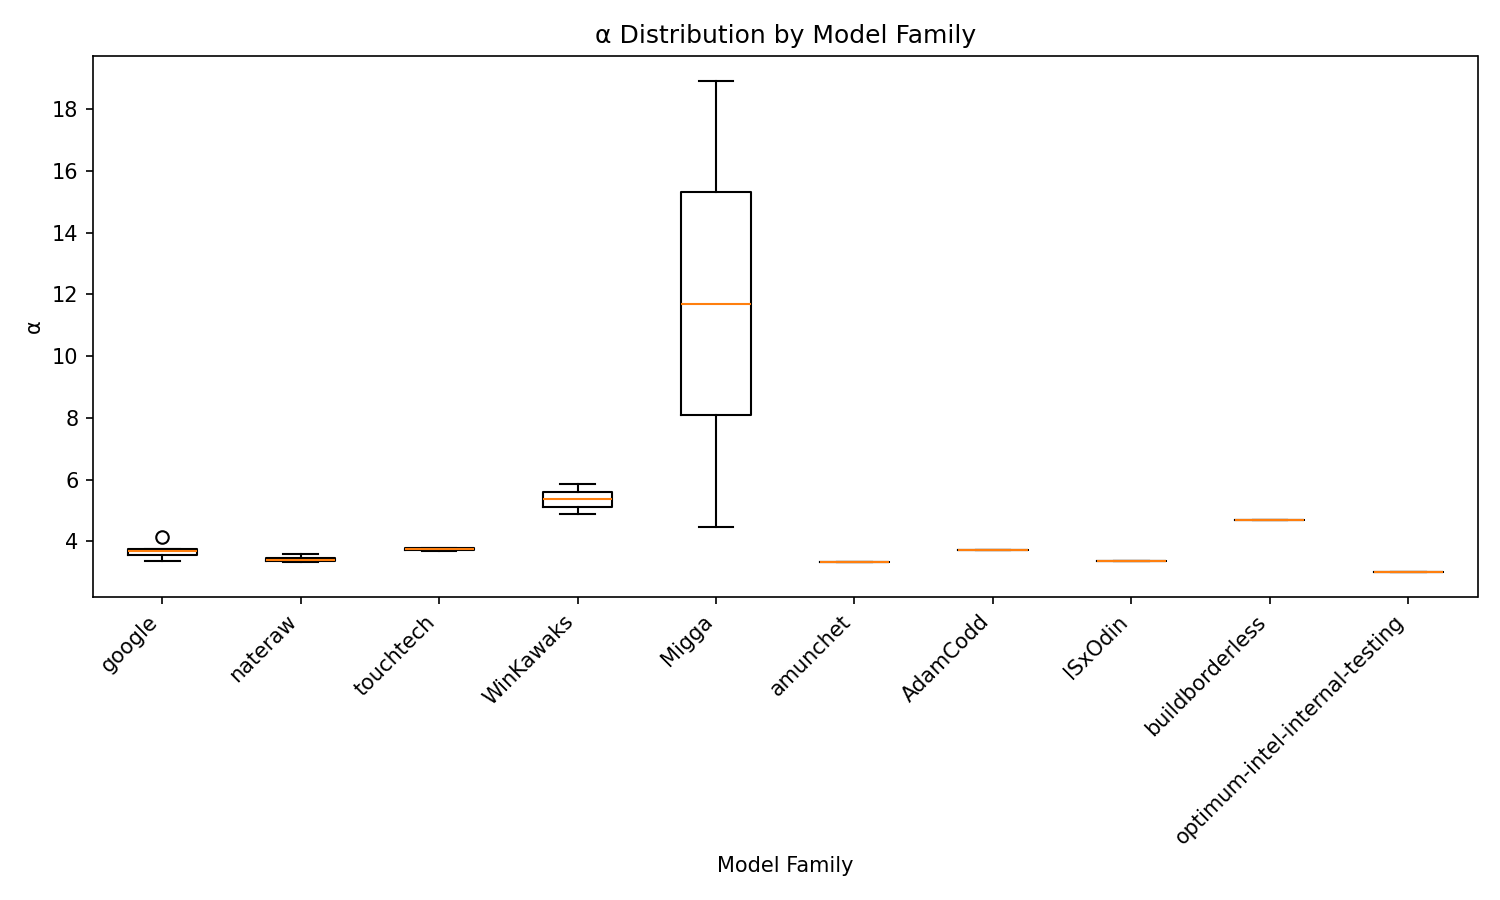
\includegraphics[width=\columnwidth]{figures/family_boxplot.png}
\caption{Family Boxplot}
\label{fig:family_boxplot}
\end{figure}

